% \part{Java}

% ----------------------------------------------------------------------------
\section{OOP mit Java}
\subsection{Exkurs}
\begin{frame}[fragile]
	\frametitle{Exkurs}
\huge Exkurs
\end{frame}

\begin{frame}
	\frametitle{Java - Von der \"Ubersetzung zur Ausf\"uhrung}
	\center
	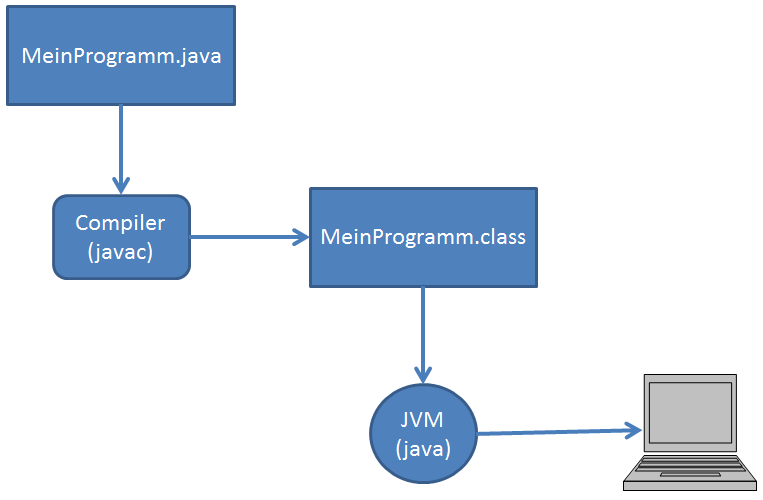
\includegraphics[width=0.8\textwidth,
	keepaspectratio=true]{bilder/java_process.png}
\end{frame}

\begin{frame}[fragile]
	\frametitle{Aufbau von Java-Dateien}
	\begin{columns}
		\begin{column}{0.5\textwidth}
			\small
			\begin{itemize}
			  \item Jede .java Datei enth\"alt eine Klassendefinition
			  \item Wichtig: \\
			  		Dateiname = Klassenname
			  \item Klassen enthalten Methoden
			  \item Methoden enthalten Anweisungen
			\end{itemize}
			\normalsize
		\end{column}
		\begin{column}{0.5\textwidth}{\tiny \itshape Test.java}
			\begin{lstlisting}
				//Klassendefinition
				class Test {
					// Der Methodenkopf
					void test(){
						//Eine Anweisung
						System.out.println("Dies ist ein Test");
					}
				}
			\end{lstlisting}
		\end{column}
	\end{columns}
\end{frame}

\begin{frame}[fragile]
	\frametitle{Aufbau von Java-Dateien}
	\begin{columns}
		\begin{column}{0.5\textwidth}
			\small
			\begin{itemize}
			  \item Programm besteht (meistens) aus mehreren Klassen
			  \item Eine Klasse beeinhaltet eine Main-Methode
			  \item JVM startet Main-Methode
			  \item Programm endet nach Ablauf der Main-Methode
			\end{itemize}
			\normalsize
		\end{column}
		\begin{column}{0.5\textwidth}{\tiny \itshape TestMitMain.java}
			\begin{lstlisting}
				class TestMitMain {
					public static void main(String[] args){
						System.out.println("Dies ist ein Test");
					}
				}
			\end{lstlisting}
		\end{column}
	\end{columns}
\end{frame}

\begin{frame}[fragile]
	  \frametitle{Methoden}
		 \begin{columns}
		 \begin{column}{0.5\textwidth}
			  \small
			  Methoden besitzen:
			  \begin{enumerate}
			  	\item Einen Methodennamen
			  	\item Anweisungen
			  	\item Lokale Variablen
			  	\item 0..* Parameter
			  	\item 0..1 R\"uckgabewerte (ohne R\"uckgabe: void)
			  	\item Wenn R\"uckgabewert dann ''return wert;''
			  	\item Zugriff auf Klassenattribute
			  	\item K\"onnen \"uberladen werden
			  \end{enumerate}
		 \end{column}
		 \begin{column}{0.5\textwidth}
		 	\begin{lstlisting}
		 		Rueckgabetyp Methodenname (Typ Parameter, ...){
		 			Anweisung1;
		 			...
		 			AnweisungN;
		 			
		 			return wert;
		 		}
		 	\end{lstlisting}
		 \end{column}
		 \end{columns}
\end{frame}

\begin{frame}[fragile]
	\frametitle{Datentypen}
	\small
	\begin{itemize}
	  \item Java enth\"alt 8 primitive Datentypen
	  \item Primitive Datentypen sind keine Objekte
	\end{itemize}
	\begin{table}
	\begin{tabular}{l|l|l}
	Name & Wertebereich & Standard\\ \hline
	byte  & -128 bis 127 & 0 \\ 
	short & -32768 bis 32767 & 0 \\
			int & -2147483648 bis 2147483647 & 0 \\
			long & $-2^{63}$ bis $2^{63}-1$ & 0 \\
			float & +/-3.40282347*1038 & 0.0 \\
			double & +/-1.79769313486231570*10308 & 0.0 \\
			char & Unicode-Zeichen & u0000 \\
			boolean& false, true & false \\
	\end{tabular}
	\end{table}
	\normalsize
\end{frame}

\begin{frame}[fragile]
	\frametitle{Variablen}
	\begin{columns}
		\begin{column}{0.5\textwidth}
			\small
			\begin{itemize}
				\item Es gibt in Java drei Arten von Variablen
					\begin{enumerate}
					  \item Klassenvariablen
					  \item Lokale Variablen
					  \item Instanzvariablen
					\end{enumerate}
				\item Variablen haben immer einen Datentyp
			\end{itemize}
		\end{column}
		\begin{column}{0.5\textwidth}
			\begin{lstlisting}
				class Variablen {
					
					//Klassenvariable
					static boolean bool = true; 
					
					//Instanzvariable
					int i = 5; 
					
					public static void main(String[] args){ 
						
						//lokale Variable
						int i = 1;
						
					}
				}
			\end{lstlisting}
		\end{column}
	\end{columns}
\end{frame}
 
\begin{frame}
	\frametitle{Variablen}
	\begin{block}{Lebensdauer}
		\begin{itemize}
			 \item Klassenvariablen: Gesamte Programmlaufzeit
			 \item Lokale Variablen: Bis zum Ende des Methodenaufrufs
			 \item Instanzvariablen: Existenz des Objekts
		\end{itemize}
	\end{block}
	\begin{exampleblock}{Sichtbarkeit}
		\begin{itemize}
			 \item Klassenvariablen: Innerhalb der Klasse
			 \item Lokale Variablen: Innerhalb eines Blocks
			 \item Instanzvariablen: Innerhalb des Objekts
		\end{itemize}
	\end{exampleblock}
\end{frame} 

\begin{frame}[fragile]
	\frametitle{Casting}
	\begin{columns}
		\begin{column}{0.5\textwidth}
			\small
			\begin{itemize}
				\item Java kann Typen implizit casten
				\item Entwickler kann Typen explizit casten
				\item Casten in gr\"o"seren Datentyp geht implizit
				\item Casten in kleineren Datentyp explizit\\
						da Informationsverlust!
			\end{itemize}
		\end{column}
		\begin{column}{0.5\textwidth}
			\begin{lstlisting}
				int i = 10;
				
				// Cast in groesseren Typ 
				// kein Problem
				long l = i;
				
				// Cast in kleineren Typ explizit
				short s = (short) i;
			\end{lstlisting}
		\end{column}
	\end{columns}
\end{frame}
 
\begin{frame}[fragile]
	\frametitle{Operatoren und Ausdr\"ucke}
	Operatoren f\"ur numerische Datentypen:
	\begin{table}
	\begin{tabular}{l|l}
	Name & Erl\"auterung \\ \hline
	+ & Addition, pos. Vorzeichen \\
			- & Subtraktion, neg. Vorzeichen \\
			* & Multiplikation \\
			/ & Division \\
			\% & Modulo \\
			++ & Pr\"a -/ Postinkrement \\
			-{}- & Pr\"a -/ Postdekrement \\
	\end{tabular}
	\end{table}
\end{frame}

\begin{frame}[fragile]
	\frametitle{Operatoren und Ausdr\"ucke}
	Vergleichsoperatoren
	\begin{table}
		\begin{tabular}{l|l}
			Name & Erl\"auterung  \\ \hline
			== & Gleich \\
			!= & Ungleich \\
			\textless & Kleiner \\
			\textgreater & Gr\"o"ser \\
			\textless= & Kleiner gleich \\
			\textgreater= & Gr\"o"ser gleich \\
		\end{tabular}
	\end{table}
\end{frame}

\begin{frame}[fragile]
	\frametitle{Operatoren und Ausdr\"ucke}
	Logische Operatoren
	\begin{table}
		\begin{tabular}{l|l}
			Name & Erl\"auterung  \\ \hline
			\&\&  & UND (Shortcircuit) \\
			$\mid\mid$ & ODER (Shortcircuit) \\
			! & NICHT \\
			\& & UND \\
			$\mid$ & ODER \\
			\textasciicircum & Exklusiv ODER \\
		\end{tabular}
	\end{table}
\end{frame}

\begin{frame}[fragile]
	\frametitle{Operatoren und Ausdr\"ucke}
	\begin{itemize}
		\item Verkn\"upfung von Variablen und anderen Ausdr\"ucken mit Operatoren
		\item Klammern beeinflussen die Reihenfolge der Auswertung
		\item Auswerten von Teilausdr\"ucken von links nach rechts
	\end{itemize}
\end{frame}

\begin{frame}[fragile]
	\frametitle{Kontrollstrukturen - Block}
	\begin{columns}
		\begin{column}{0.5\textwidth}
			\begin{itemize}
			\item Fasst mehrere Anweisungen Zusammen
			\item Kann stehen wo auch einzelne Anweisungen stehen
			\item Kann geschachtelt werden
		\end{itemize}
		\end{column}
		\begin{column}{0.5\textwidth}
			\begin{lstlisting}
				{
					System.out.println("Ausgabe");
					System.out.println("Ausgabe");
				}
			\end{lstlisting}
		\end{column}
	\end{columns}
\end{frame}

\begin{frame}[fragile]
	\frametitle{Kontrollstrukturen - Fallunterscheidung}
	\begin{columns}
		\begin{column}{0.5\textwidth}
			\begin{itemize}
			  \item Bedingte Anweisung
			  \item Ausdruck ''Bedingung'' muss boolescher Ausdruck sein\\
			  d.h. \begin{itshape}true\end{itshape} oder
			  \begin{itshape}false\end{itshape}
			\end{itemize}
		\end{column}
		\begin{column}{0.5\textwidth}
			\begin{lstlisting}
				if(Bedingung){
					System.out.println("Die Bedingung ist True");
				}
			\end{lstlisting}
		\end{column}
	\end{columns}
\end{frame}

\begin{frame}[fragile]
	\frametitle{Kontrollstrukturen - Fallunterscheidung}
	\begin{columns}
		\begin{column}{0.5\textwidth}
			\small
			\begin{itemize}
			  \item Mehrfachauswahl
			  \item Auch hier: \\ 
			  Ausdr\"ucke ''Bedingung1'' \\
			  und ''Bedingung2'' m\"ussen boolesche Ausdr\"ucke sein\\
			  \item else-Zweig wird durchlaufen wenn kein Ausdruck wahr ist
			\end{itemize}
		\end{column}
		\begin{column}{0.5\textwidth}
			\begin{lstlisting}
				if(Bedingung1){
					System.out.println("Bedingung1 ist True");
				} else if(Bedingung2){
					System.out.println("Bedingung2 ist True");
				} else {
					System.out.println("Keine Bedingung ist True");
				}
				
				// If-Then-Else als 
				// ternaerer Operator
				Ausdruck = ( BedingungX ) ? Wahr : Falsch;
			\end{lstlisting}
		\end{column}
	\end{columns}
\end{frame}

\begin{frame}[fragile]
	\frametitle{Kontrollstrukturen - Fallunterscheidung}
	\begin{columns}
		\begin{column}{0.5\textwidth}
			\small
			\begin{itemize}
			  \item Mehrfachauswahl
			  \item Ausdruck vom Typ:\\
			  byte, short, char, int
			  \item Nach case darf genau 1 Konstante stehen
			  \item Wenn keine passende Konstante 
			  dann ''default'' Anweisung (wenn vorhanden)
			  \item Ohne break: \\
			  ausf\"uhren aller Anweisungen ab \"Ubereinstimmung
			  \item ''break'' ist syntaktisch nicht erforderlich
			\end{itemize}
		\end{column}
		\begin{column}{0.5\textwidth}
			\begin{lstlisting}
				switch(Ausdruck){
					
					case konst1:
						Anweisung1;
						break;
						
					case konst2:
						Anweisung2;
						break;
						
					default:
						Anweisung3;
						break;
						
				}
			\end{lstlisting}
		\end{column}
	\end{columns}
\end{frame}

\begin{frame}[fragile]
	\frametitle{Kontrollstrukturen - Schleifen}
	\begin{columns}
		\begin{column}{0.5\textwidth}
			\begin{itemize}
			  \item Kopfgesteuerte Schleife
			  \item Pr\"uft Ausdruck zu Beginn 
			\end{itemize}
		\end{column}
		\begin{column}{0.5\textwidth}
			\begin{lstlisting}
				while (Bedingung){
					Anweisung1;
					...
					Anweisungn;
				}
			\end{lstlisting}
		\end{column}
	\end{columns}
\end{frame}

\begin{frame}[fragile]
	\frametitle{Kontrollstrukturen - Schleifen}
	\begin{columns}
		\begin{column}{0.5\textwidth}
			\begin{itemize}
			  \item Fu"sgesteuerte Schleife
			  \item Pr\"uft Ausdruck am Ende der Schleife 
			\end{itemize}
		\end{column}
		\begin{column}{0.5\textwidth}
			\begin{lstlisting}
				do{
					Anweisung1;
					...
					Anweisungn;
				}while (Bedingung);
			\end{lstlisting}
		\end{column}
	\end{columns}
\end{frame}

\begin{frame}[fragile]
	\frametitle{Kontrollstrukturen - Schleifen}
	\begin{columns}
		\begin{column}{0.5\textwidth}
			\begin{itemize}
				  \item Z\"ahlschleife
				  \item Auch Kopfgesteuert
				  \item ''Initial'' wird vor 1. Durchlauf ausgewertet
				  \item ''Bedingung'' wird vor jedem Durchlauf ausgewertet
				  \item ''Inc/Dec'' wird nach jedem Durchlauf ausgewertet
				\end{itemize}
			\end{column}
		\begin{column}{0.5\textwidth}
			\begin{lstlisting}
				for(Initial; Bedingung; Inc/Dec)
				{
					Anweisung1;
					...
					AnweisungN;
				}
			\end{lstlisting}
		\end{column}
	\end{columns}
\end{frame}

\begin{frame}[fragile]
	  \frametitle{Arrays}
		 \begin{columns}
		 \begin{column}{0.5\textwidth}
			  \small
			  \begin{itemize}
			    \item Arrays fassen Variablen mit gleichem Typ
			    zusammen
			    \item Zugriff via Index
			    \item Array ist ein Objekt
			    \item Kann primitiven Datentyp 
			    oder Objektreferenzen enthalten
			    (nicht ver\"anderbar)
			    \item Elementanzahl wird in public Attribut
			    ''length'' gespeichert
			    \item Kann mehrdimensional sein
			  \end{itemize}
		 \end{column}
		 \begin{column}{0.5\textwidth}
		 	\begin{lstlisting}
		 		// Array deklarieren
		 		int[] noten;
		 		
		 		// Int-Array erzeugen
		 		// Mit Platz fuer 25
		 		// Elemente
		 		noten = new int[25];
		 		
		 		// Werte zuweisen
		 		// Erste Element an
		 		// Stelle 0
		 		noten[0] = 5;
		 		noten[1] = 4;
		 		noten[2] = 6;
		 		
		 		// Auch moeglich
		 		// Array mit 3 Elementen
		 		int[] ar = {1,4,5};
		 		
		 		// Mehrdimensionales Array
		 		int[][] tabelle = new int[4][4];
		 		
		 	\end{lstlisting}
		 \end{column}
		 \end{columns}
\end{frame}

\begin{frame}[fragile]
	  \frametitle{Strings}
		 \begin{columns}
		 \begin{column}{0.5\textwidth}
			  \small
			  \begin{itemize}
			    \item Strings sind Objekte
			    \item K\"onnen ohne ''new'' angelegt werden
			    \item Konstruktoren existieren auch
			    \item Strings sind immutable\\
			    (nicht ver\"anderbar)
			    \item \"Andern eines Zeichens erzeugt neuen
			    String
			    \item Vergleich mit equals-Methode
			  \end{itemize}
		 \end{column}
		 \begin{column}{0.5\textwidth}
		 	\begin{lstlisting}
		 		// Erstellen ohne ''new''
		 		String farbe = "rot";
		 		String farbe2 = "blau";
		 		
    			// Klasse hat viele Methoden
    			// Hier 3 Beispiele,
    			// mehr sind in der API-Doku

		 		// Gibt die Laenge zurueck
		 		int laenge = farbe.length();
		 		
		 		// Gibt das Zeichen 
		 		// an Position 2
		 		// zurueck
		 		// Wichtig: 1. Zeichen
		 		// steht an Position 0
		 		char c = farbe.charAt(2);
		 		
		 		// Ein Vergleich
		 		// Ergebnis: false
		 		farbe.equals(farbe2);
		 		
		 		// Noch ein Vergleich
		 		// Ergebnis: true
		 		"blau".equals(farbe2);
		 	\end{lstlisting}
		 \end{column}
		 \end{columns}
\end{frame}

\begin{frame}[fragile]
	  \frametitle{Strings}
		 \begin{columns}
		 \begin{column}{0.5\textwidth}
			  \small
			  \begin{itemize}
			    \item ''+''-Operator f\"ugt Strings zusammen
			    \item Andere Datentypen werden beim
			    Zusammenf\"ugen automatisch
			    in Strings umgewandelt
			  \end{itemize}
		 \end{column}
		 \begin{column}{0.5\textwidth}
		 	\begin{lstlisting}
		 		// String concat
		 		String a = "rot";
		 		String b = "blau";
		 		String c = "gruen";
		 		System.out.println(a+b+c);
		 		
		 		// Umwandlung in String
		 		int i = 10;
		 		String prefix = "Geld: ";
		 		String postfix = "Euro";
		 		String message = prefix + i + postfix;
		 		System.out.println(message);
		 	\end{lstlisting}
		 \end{column}
		 \end{columns}
\end{frame}

\begin{frame}
	\frametitle{Zeit f\"ur eine \"Ubung}
	\center
	
\includegraphics[width=0.8\textwidth,
	keepaspectratio=true]{bilder/uebung.png}
\end{frame}

\subsection{Klassen und Objekte}
\begin{frame}[fragile]
	\frametitle{Klassen und Objekte}
	\huge Klassen und Objekte
\end{frame}

\begin{frame}[fragile]
	\frametitle{Klassen in Java}
	\begin{columns}
		\begin{column}{0.5\textwidth}
			\small
			Vereinfachung der Kuh-Klasse:
			\center
			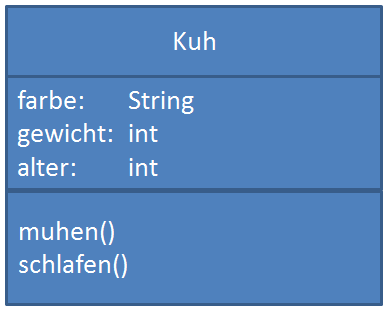
\includegraphics[width=0.8\textwidth,
			keepaspectratio=true]{bilder/klasse_ohne_kuh.png}
		\end{column}
		\begin{column}{0.5\textwidth}
			\begin{lstlisting}
				public class Kuh
				{
					private int alter;
					private int gewicht;
					private String farbe;
					
					public void muhen(){
						System.out.println("Muh");
					}
					
					public void schlafen(){
						...
					}
				} 
			\end{lstlisting}
		\end{column}
	\end{columns}
\end{frame}

\begin{frame}[fragile]
	\frametitle{Klassen in Java}
	\begin{columns}
		\begin{column}{0.5\textwidth}
			\small
			\begin{itemize}
			  \item Eine Java-Klasse besteht aus:\\
			  \begin{enumerate}
			  	\item Klassennamen
			  	\item Konstruktoren
			  	\item Methoden
			  	\item Attributen\\
			  	(Instanz- / Klassenvariablen)
			  \end{enumerate} 
			\end{itemize}
		\end{column}
		\begin{column}{0.5\textwidth}
			\begin{lstlisting}
				Modifier class Klassenname{
					//Haben Typ und Variablennamen
					Attribute
					
					// Spezielle Methoden die nach
					// der Instanziierung aufgerufen
					// werden
					Konstruktoren
					
					// Besitzen ggf. Parameter und 
					// Rueckgabewert
					Methoden
				}
			\end{lstlisting}
		\end{column}
	\end{columns}
\end{frame}

\begin{frame}[fragile]
	\frametitle{Modifier}
	\begin{itemize}
	  \item Kann Klassen, Methoden, 
	  Attributen vorangestellt werden
	  \item Hat Einfluss auf:
	  \begin{enumerate}
	  	\item Sichtbarkeit
	  	\item Lebensdauer
	  	\item Modifikation
	  \end{enumerate}
	  \item Attribute sind private (Geheimnisprinzip)
	  \item Beispiele:
	  \begin{enumerate}
	  	\item public
	  	\item private
	  	\item final
	  	\item \ldots
	  \end{enumerate}
	\end{itemize}
\end{frame}

\begin{frame}[fragile]
	  \frametitle{Sichtbarkeit}
		 \begin{columns}
		 \begin{column}{0.5\textwidth}
			  \small
			  \begin{itemize}
			    \item 3 Modifier beeinflussen die Sichtbarkeit:
			  	\begin{enumerate}
			  	  \item private
			  	  \item protected
			  	  \item public
			  	\end{enumerate}
			  	\item Default ist ''package''
			  \end{itemize}
		 \end{column}
		 \begin{column}{0.5\textwidth}
		 	\begin{lstlisting}
		 		// Nur innerhalb der 
		 		// eigenen Klasse sichtbar
		 		private int alter;
		 		
		 		// Sichtbar fuer abgeleitete
		 		// Klassen und Klasesn im 
		 		// selben Package
		 		protected int gewicht;
		 		
		 		// Ueberall sichtbar
		 		// Nur Public-Klassen koennen
		 		// ausserhalb des eigenen Pakets
		 		// genutzt werden
		 		public String farbe;
		 	\end{lstlisting}
		 \end{column}
		 \end{columns}
\end{frame}

\begin{frame}[fragile]
	  \frametitle{Modifier ''final''}
	  \begin{columns}
		  \begin{column}{0.5\textwidth}
			  \small
			  \begin{itemize}
			  	\item Anwendung auf:
			  	\begin{enumerate}
			  	  \item Methoden
			  	  \item Variablen
			  	  \item Klassen\\
			  	\end{enumerate}
			  	\item Verhindert die nachtr\"agliche
			  	 Ver\"anderung
			  	 \item Konstanten = static + final 
			  	 Attribute
			  \end{itemize}
		  \end{column}
		  \begin{column}{0.5\textwidth}
		  	\begin{lstlisting}
		  		// final auf Klassenebene verhindert 
		  		// das Erben von Kuh
			  	public final class Kuh{
			  		...
			  		// Kann nur 1 mal beim
			  		// direkten Initialisieren
			  		// oder im Konstruktor
			  		// gesetzt werden 
			  		private final String farbe;
			  		...
			  		// Kann nicht durch Vererbung 
			  		// veraendert werden
			  		public final void muhen(){
			  			...
			  		}
		  	\end{lstlisting}
		  \end{column}
	  \end{columns}
\end{frame}

\begin{frame}[fragile]
	  \frametitle{Packages}
	  \small
	  \begin{itemize}
	  	\item Klassen werden in Paketen verwaltet
		  	\begin{enumerate}
		  	  \item Zur besseren Darstellung der Struktur
		  	  \item Zur Vermeidung von Namenskonflikten
		  	  \item Zur Zugriffsbeschr\"ankung
		  	\end{enumerate}
		\item Jede Klasse liegt im thematisch passenden
		Package
	  \end{itemize}
\end{frame}

\begin{frame}[fragile] 
	  \frametitle{Packages}
		 \begin{columns}
		 \begin{column}{0.5\textwidth}
			  \small
			  \begin{itemize}
			  	\item Imports
				  	\begin{enumerate}
				  	  \item Eingabe des FQN ist umst\"andlich
				  	  \item L\"osung: Import-Anweisung
				  	  \item Imports am Anfang jeder Java-Datei
				  	  \item macht Angabe des FQN \"uberfl\"ussig
				  	\end{enumerate}
				\item Paket java.lang wird automatisch
				importiert
			  \end{itemize}
		 \end{column}
		 \begin{column}{0.5\textwidth}
		 	\begin{lstlisting}
		 		// Wenn mehr aus Util 
		 		// verwendet wird:
		 		// import java.util.*;
		 		import java.util.Calendar;
		 		
		 		public class HatKalender{
		 		 	//statt: java.util.Calendar c = ...;
		 			Calendar c = Calendar.getInstance();
		 		}
		 	\end{lstlisting}
		 \end{column}
		 \end{columns}
\end{frame}

\begin{frame}[fragile]
	\frametitle{Packages}
	Mit Java mitgelieferte Pakete:\\
	(Auszug, es gibt weit mehr!)
	\begin{table}
		\begin{tabular}{l|l|l}
			Name & Wertebereich \\ \hline
			java.lang  & Basiskonstrukte \\ 
			java.util & Hilfsklassen (Datenstrukturen etc\ldots)  \\
			java.io & Input-/Output \\
			javax.swing & GUI 
		\end{tabular}
	\end{table}
	\normalsize
\end{frame}

\begin{frame}[fragile]
	  \frametitle{Packages}
		 \begin{columns}
		 \begin{column}{0.5\textwidth}
			  \small
			  \begin{itemize}
			  	\item Eigene Klasse wird mit ''package'' 
			  	in ein Paket gepackt
			  	\item Steht als als erstes (!) in jeder Java-Datei
			  	\item Namen immer klein geschrieben
			  	\item Java-Dateien liegen in 
			  	entsprechendem Verzeichnis
			  	\item Ohne Angabe landet Klasse in Default-Paket
			  	(aktuelles Verzeichnis)
			  \end{itemize}
		 \end{column}
		 \begin{column}{0.5\textwidth}
		 	\begin{lstlisting}
		 		// Ab jetzt liegt unsere 
		 		// Klasse im Package
		 		// Wichtig: Im Filesystem
		 		// liegt die Klasse nun auch 
		 		// unter: 
		 		// ./com/fom/oop/bauernhof
		 		package com.fom.oop.bauernhof;
		 		
		 		// Alle Imports die 
		 		// wir benoetigen
		 		import ...;
		 		...
		 		
		 		public class Kuh{
		 			...
		 		}
		 	\end{lstlisting}
		 \end{column}
		 \end{columns}
\end{frame}

\begin{frame}[fragile]
	\frametitle{Objekte in Java}
	\begin{columns}
		\begin{column}{0.5\textwidth}
			\small
			\begin{itemize}
			  \item Objekte werden mit dem Operator ''new'' erzeugt
			  \item Objekte werden dynamisch auf Heap erzeugt
			  \item Variablen k\"onnen Referenzen auf Objekte aufnehmen\\
			  		Nicht die Objekte selbst!
			\end{itemize}
		\end{column}
		\begin{column}{0.5\textwidth}
			\begin{lstlisting}
				// Variable vom Typ Kuh
				// Kann eine Referenz auf
				// ein Kuh-Objekt aufnehmen
				Kuh milkaKuh;
				
				// Neues Objekt erzeugen und
				// Referenz der Variable zuweisen
				milkaKuh = new Kuh();
			\end{lstlisting}
		\end{column}
	\end{columns}
\end{frame}

\begin{frame}[fragile]
	\frametitle{Objekte in Java}
	Ein Objekt der Klasse Kuh:
	\begin{columns}
		\begin{column}{0.5\textwidth}
			\small
			\begin{itemize}
			  \item Attribute sind private
			  \item Nur Zugriff auf Objektmethoden m\"oglich
			  \item Attribute der Klasse sind nicht initialisiert\\
			  Standardwerte: alter = 0, gewicht = 0, farbe = null
			  \item Attribute setzen durch:\\
			  Methoden oder Konstruktor
			\end{itemize}
		\end{column}
		\begin{column}{0.5\textwidth}
		\small Unser Kuh-Bauplan:
			\begin{lstlisting}
				public class Kuh
				{
					private int alter;
					private int gewicht;
					private String farbe;
					
					public void muhen(){
						System.out.println("Muh");
					}
					
					public void schlafen(){
						...
					}
				} 
			\end{lstlisting}
		\end{column}
	\end{columns}
\end{frame}

\begin{frame}[fragile]
	\frametitle{Konstruktoren}
	\begin{columns}
		\begin{column}{0.5\textwidth}
			\small
			\begin{itemize}
			  \item Spezielle Methode
			  \item Wird direkt nach Objekterzeugung aufgerufen
			  \item Gleicher Name wie Klasse
			  \item 0..* Parameter
			  \item Kein R\"uckgabewert
			  \item Klassen kann mehrere Konstruktoren besitzen
			  \item Besitzt Klasse keinen Konstruktor wird 
			  default-Konstruktor aufgerufen
			\end{itemize}
		\end{column}
		\begin{column}{0.5\textwidth}
			\begin{lstlisting}
				public class Kuh
				{
					private int alter;
					private int gewicht;
					private String farbe;
					
					//Konstruktor  
					public Kuh(int a, int g, String f){
						alter = a;
						gewicht = g;
						farbe = f;
					}
					
					//Konstruktor  
					public Kuh(int a, int g){
						alter = a;
						gewicht = g;
						farbe = "Schwarz-Weiss";
					}
					
					public void muhen(){
						System.out.println("Muh");
					}
					
					public void schlafen(){
						...
					}
				} 
			\end{lstlisting}
		\end{column}
	\end{columns}
\end{frame}

\begin{frame}[fragile]
	\frametitle{Initialisierung mit Konstruktoren}
	\begin{columns}
		\begin{column}{0.5\textwidth}
			\small
			\begin{itemize}
			  \item Konstruktor wirkt sich auf Art der 
			  Instanziierung auf
			  \item Ohne parameterlosen Konstruktur m\"ussen 
			  bei ''new'' Parameter \"ubergeben werden\\
			  (gem\"a"s Konstruktoren)
			\end{itemize}
		\end{column}
		\begin{column}{0.5\textwidth}
			\begin{lstlisting}
				// Deklaration der Variable
				Kuh elsa;
				
				// Intanziieren des Objekts
				elsa = new Kuh(10, 350, "lila");
				
				// Intanziieren des Objekts
				elsa = new Kuh(10, 350);
			\end{lstlisting}
		\end{column}
	\end{columns}
\end{frame}

\begin{frame}[fragile]
	\frametitle{Methodenaufrufe}
	\begin{columns}
		\begin{column}{0.6\textwidth}
			\small
			\begin{itemize}
			  \item Durch Methodenaufruf wird Objekt 
			  eine Nachricht geschickt
			  \item Aufruf:\\
			  Referenzvariable.\\
			  Methodenname(Parameter\ldots);
			\end{itemize}
		\end{column}
		\begin{column}{0.4\textwidth}
			\begin{lstlisting}
				// Deklaration der Variable
				Kuh elsa;
				
				// Intanziieren des Objekts
				elsa = new Kuh(10, 350, "lila");
				
				// Aufruf von Objektmethoden
				elsa.schlafen();
				elsa.muhen();
			\end{lstlisting}
		\end{column}
	\end{columns}
\end{frame}

\begin{frame}[fragile]
	\frametitle{Objekterzeugung}
	\begin{columns}
		\begin{column}{0.5\textwidth}
			\small
			\begin{itemize}
			  \item Von einer Klasse k\"onnen mehrere Objekte erzeugt werden
			  \item Jedes Objekt ist individuell auch wenn die Attribute
			  die selbern Werte haben
			  \item Achtung: \\
			  Beim Vergleich werden die Referenzen verglichen
			\end{itemize}
		\end{column}
		\begin{column}{0.5\textwidth}
			\begin{lstlisting}
				// Unsere Elsa
				Kuh elsa = new Kuh(10,350, "lila");
				
				// Unsere Bertha
				Kuh bertha = new Kuh(10, 350, "lila");
				
				// Vergleich liefert
				// false zurueck
				if(elsa == bertha){
					...
				} 
			\end{lstlisting}
		\end{column}
	\end{columns}
\end{frame}

\begin{frame}[fragile]
	\frametitle{Getter und Setter}
	\begin{columns}
		\begin{column}{0.5\textwidth}
			\small
			\begin{itemize}
			  \item Unsere Kuh bekommt das Feld ''anzBesuchteHoefe''
			  \item ''anzBesuchteHoefe'' ist private
			  \item F\"ur Zugriff werden get-/set-Methoden implementiert
			  \item Setter \"andert den Wert des betroffenen Attributs
			  \item Getter gibt aktuellen Wert zur\"uck
			  \item Namen der Methoden beginnen mit ''get'' oder ''set''
			\end{itemize}
		\end{column}
		\begin{column}{0.5\textwidth}
			\begin{lstlisting}
				public class Kuh
				{
					private int alter;
					private int gewicht;
					private String farbe;
					private int anzBesuchteHoefe;
					
					//Konstruktor  
					public Kuh(int a, int g, String f){
						alter = a;
						gewicht = g;
						farbe = f;
					}
					
					//Konstruktor  
					public Kuh(int a, int g){
						alter = a;
						gewicht = g;
						farbe = "Schwarz-Weiss";
					}
					
					public int getAnzBesuchteHoefe(){
						return anzBesuchteHoefe;
					}
					
					public void setAnzBesuchteHoefe(int anz){
						this.anzBesuchteHoefe = anz;
					}
					...
				} 
			\end{lstlisting}
		\end{column}
	\end{columns}
\end{frame}

\begin{frame}[fragile]
	\frametitle{Getter und Setter}
	\begin{columns}
		\begin{column}{0.5\textwidth}
			\small
			\begin{itemize}
			  \item Setter \"andert Objektzustand
			  \item ''this'' ist Referenz auf das Objekt selbst
			  \item Durch ''this'' k\"onnen Objektvariablen 
			  verwendet werden, die durch lokale \"uberdeckt sind
			\end{itemize}
		\end{column}
		\begin{column}{0.5\textwidth}
			\begin{lstlisting}
				// Unsere Kuh Elsa
				Kuh elsa = new Kuh(10, 350);
				
				// Elsa hat schon 5 Hoefe besucht
				elsa.setAnzBesuchteHoefe(5);
				
				// Ausgabe der Anzahl
				System.out.println(elsa.getAnzBesuchteHoefe());
				
			\end{lstlisting}
		\end{column}
	\end{columns}
\end{frame}

\begin{frame}[fragile]
	  \frametitle{Modifier ''static''}
		 \begin{columns}
		 \begin{column}{0.5\textwidth}
			  \small
			  Statische Methoden:
			  \begin{itemize}
			  	\item Implementiert Verhalten unabh\"angig
			  	von Objektzustand
			  	\item Z.B. f\"ur mathematische Funktionen
			  	\item Objekt in dem Fall nicht sinnvoll
			  	\item Steht ab Laden der Klasse bis Ende des
			  	Programms zur Verf\"ugung
			  	\item Nicht an Objektexistenz gebunden
			  	\item Beispiel: Main-Methode
			  	\item Aufruf \"uber Klassenname
			  \end{itemize}
		 \end{column}
		 \begin{column}{0.5\textwidth}
		 	\begin{lstlisting}
		 		public class MatheLib {
		 			// Privater Konstruktor
		 			// Instanziierung nicht
		 			// mglich
		 			private MatheLib(){}
		 			
		 			// Static Methode
		 			// kann auch ohne Objekt
		 			// aufgerufen werden
		 			public static int sum(int z1, int z2){
		 				return z1+z2;
		 			}
		 		}
		 	\end{lstlisting}
		 	
		 	\begin{lstlisting}
		 		// Aufruf
		 		// summe = 2
		 		int summe = MatheLib.sum(1,1);
		 	\end{lstlisting}
		 \end{column}
		 \end{columns}
\end{frame}

\begin{frame}[fragile]
	  \frametitle{Modifier ''static''}
		  \small
		  Statische Attribute:
		  \begin{itemize}
		    \item Klassenvariablen
		  	\item Nicht an Objekte gebunden
		  	\item Klassenvariablen werden von allen
		  	Objektinstanzen geteilt
		  	\item Verwendung: z.B. als Objektz\"ahler
		  	\item Initialisierung vor Objekterzeugung
		  	\item Initialisierung vor Aufruf statischer
		  	Methoden
		  \end{itemize}
\end{frame}

\begin{frame}[fragile]
	  \frametitle{Modifier ''static''}
		 \begin{alertblock}{Zu Beachten}
			  \begin{itemize}
			  	\item Keine Aufrufe von non-static
			  	 Methoden aus static Methoden heraus
			  	\item Keine Verwendung von non-static
			  	 Objektvariablen innerhalb von static Methoden
			  \end{itemize}
		  \end{alertblock}
\end{frame}

\begin{frame}
	\frametitle{Zeit f\"ur eine \"Ubung}
	\center
	
\includegraphics[width=0.8\textwidth,
	keepaspectratio=true]{bilder/uebung.png}
\end{frame}

\subsection{Vererbung} 
\begin{frame}[fragile]
	\frametitle{Vererbung}
	\huge Vererbung
\end{frame}

\begin{frame}[fragile]
	\frametitle{Vererbung mit Java}
		\begin{itemize}
		  \item Abgeleitete Klasse erbt
		  alle non-private Eigenschaften
		  \item Geerbte Methoden k\"onnen
		  \"uberschrieben werden
		  \item Abgeleitete Klasse kann
		  zus\"atzliche Methoden enthalten
		  \item eine Klasse erbt mit dem
		  Keyword ''extends''
		  \item Konstruktor der Basisklasse
		  muss aufgerufen werden
		\end{itemize}
\end{frame} 

\begin{frame}[fragile]
	\frametitle{Vererbung und Konstruktoren}
	\begin{columns}
		\begin{column}{0.5\textwidth}
		Default-Konstruktor:
		\begin{lstlisting}
			public class Kuh{
				private int alter;
				private int gewicht;

				public void muhen(){
					System.out.println("Muh!");
				}
			} 
			
			public class SuperKuh extends Kuh{
				// Ueberschreiben der
				// Methode von Kuh
				public void muhen(){
					System.out.println("Supermuh!!!!");
				}
				
				// Neue Methode
				public void fliegen()
					// fliegen
				}
			}
			\end{lstlisting}
		\end{column}
		\begin{column}{0.5\textwidth}
		Spezifischer Konstruktor:
		\begin{lstlisting}
			public class Kuh{
				private int alter;
				private int gewicht;
				
				public Kuh(int alter, int gewicht){
					this.alter = alter;
					this.gewicht = gewicht;
				}
				...
			}
			
			public class SuperKuh extends Kuh{
				// Parameter duerfen sich
				// unterscheiden, jedoch
				// muss Konstruktor der Vaterklasse
				// aufgerufen werden
				public SuperKuh(){
					super(5,350);
				}
				...
			}
			\end{lstlisting}
		\end{column}
	\end{columns}
\end{frame} 

\begin{frame}[fragile]
	\frametitle{Vererbung und Eigenschaften}
		\begin{itemize}
		  \item Automatischer Aufruf des 
		  Default-Konstruktors (wenn kein spezieller)
		  \item Superkuh kann nicht direkt
		  auf Variablen von Kuh zugreifen
		  \item Zugriff nur \"uber public 
		  Methoden
		  \item Die Methode ''muhen'' wird 
		  \"uberschrieben
		  \item Die Methode fliegen() gibts 
		  nur bei Superk\"uhen
		\end{itemize}
\end{frame}

\begin{frame}[fragile]
	\frametitle{\"Uberschreiben vs \"Uberladen}
		\begin{exampleblock}{\"Uberschreiben}
			\begin{itemize}
			  \item Methodensignatur ist in Vater- und Kindklasse
			  gleich
			  \item Abgeleitete Klasse des urspr\"unglichen
			  return-Werts m\"oglich
			  \item Sichtbarkeit darf nicht eingeschr\"ankter werden
			  \item Nutzung bei Vererbung
			\end{itemize}
		\end{exampleblock}
		
		\begin{alertblock}{\"Uberladen}
			\begin{itemize}
			  \item Methoden mit gleichen Namen in Klasse
			  \item Methoden unterscheiden sich hinsichtlich
			  Parameter
			  \item R\"uckgabewerte k\"onnen unterschiedlich sein
			  \item Sichtbarkeit kann sich \"andern
			\end{itemize}
		\end{alertblock}  
\end{frame}

\begin{frame}[fragile]
	\frametitle{Vererbungsstufen}
			\begin{itemize}
			  \item Vererbungsstufen sind nicht
			  begrenzt
			  \item Von SuperKuh kann wieder geerbt 
			  werden
			  \item Jede Kind-Klasse erbt alle
			  Eigenschaften aus ihrer Hierarchie
			  (Gesetz den Vorgaben von Java)
			  \item Von Klassen kann auch mehrfach 
			  geerbt werden (MilkaKuh erbt von Kuh)
			  \item Vererbung beschreibt eine ''ist eine''
			  - Beziehung
			  \item Eine Superkuh ist eine Kuh\\
			 (Aber nicht jede Kuh ist eine Superkuh)
		\end{itemize}
\end{frame} 

\begin{frame}[fragile]
	\frametitle{Die Klasse Object}
			\begin{itemize}
			  \item Alle Klassen erben automatisch von Object
			  \item Erbt eine Klasse von niemanden wird ''extends
			  Object'' implizit angef\"ugt
			  \item Von Object geerbte Methoden:
			  \begin{enumerate}
			    \item boolean equals(Object obj)
			    \item protected Object clone()
			    \item String toString()
			    \item int hashCode()
			  \end{enumerate}
		\end{itemize}
\end{frame} 

\begin{frame}[fragile]
	\frametitle{Vorteile}
		\begin{exampleblock}{Vorteile von Vererbung}
			\begin{itemize}
			  \item Bessere Wartbarkeit
			  \item F\"ordert Wiederverwendung
			  \item Bessere Erweiterbarkeit
			\end{itemize}
		\end{exampleblock} 
\end{frame}

\begin{frame}
	\frametitle{Zeit f\"ur eine \"Ubung}
	\center
	
\includegraphics[width=0.8\textwidth,
	keepaspectratio=true]{bilder/uebung.png}
\end{frame}

\subsection{Polymorphismus}
\begin{frame}[fragile]
	\frametitle{Polymorphismus}
	\huge Polymorphismus
\end{frame}

\begin{frame}[fragile] 
	\frametitle{Polymorphismus} 
	\begin{columns}
		\begin{column}{0.5\textwidth}
			\begin{itemize}
			  \item Die Kindklasse kann \"uberall dort benutzt 
			  werden wo auch die Vaterklasse genutzt wird
			  \item W\"ahrend des Kompilierens steht nicht fest
			  welche Methode ausgef\"uhrt wird
			  \item Es kann Methode der Basisklasse sein, oder eine
			  einer Kindklasse
			\end{itemize}
		\end{column}
		\begin{column}{0.5\textwidth}
			\begin{lstlisting}
				// Kuh-Referenz zeigt auf 
				// SuperKuh-Objekt
				Kuh hilde = new SuperKuh();
				
				// Es wird das ''muhen''
				// einer SuperKuh ausgefuehrt
				// Ausgabe: Supermuh!!!
				hilde.muhen();
			\end{lstlisting}
		\end{column}
	\end{columns}
\end{frame}

\begin{frame}[fragile]
	\frametitle{M\"oglichkeiten des Polymorphismus}
		\begin{itemize}
		  \item Kein Wissen \"uber konkrete Klasse oder
		  Implementierung von Methoden n\"otig
		  \item Unterschiedliche Methoden f\"ur gleiche
		  Referenztypen
		  \item Wichtig f\"ur Erweiterbarkeit
		\end{itemize}
\end{frame}

\begin{frame}[fragile]
	\frametitle{Polymorphismus, Referenzen und Methodenaufrufe}
	\begin{columns}
		\begin{column}{0.5\textwidth}
			\begin{itemize}
			  \item Compiler checkt den Referenztyp
			  nicht das Objekt
			  \item Daher k\"onnen nur Methoden
			  aufgerufen werden, die der Referenz-Klasse
			  angeh\"oren
			  \item L\"osung: Casting
			\end{itemize}
		\end{column}
		\begin{column}{0.5\textwidth}
			\begin{lstlisting}
				// Es koennen nur Methoden
				// der Kuh-Klasse aufgerufen 
				// werden
				Kuh hilde = new SuperKuh();
				
				// Compiler wirft einen Fehler
				hilde.fliegen();
				
				// Um den Fehler zu vermeiden
				// Casten wir unsere Hilde
				SuperKuh superHilde = null;
				if(hilde instanceof SuperKuh){
					superHilde = (SuperKuh) hilde;
				}
				superHilde.fliegen();
			\end{lstlisting}
		\end{column}
	\end{columns}
\end{frame}

\begin{frame}[fragile]
	\frametitle{Polymorphismus, Referenzen und Methodenaufrufe}
		\begin{alertblock}{Achtung}
			\begin{itemize}
			  \item Referenz der Kindklasse auf die abgeleitete Klasse
			  funktioniert nicht
			  \item Fehler:\\
			  SuperKuh heldin = new Kuh();
			  \item Der Objekttyp kann die Methoden des Referenztyps
			  nicht bedienen
			\end{itemize}
		\end{alertblock}  
\end{frame}

\begin{frame}[fragile]
	\frametitle{Dynamisches vs. Statisches Binding}
		\begin{block}{Dynamisches Binding}
			\begin{itemize}
			  \item Da Methode nicht bei Kompilierung bestimmt werden kann
			  muss JVM sie zur Laufzeit suchen
			  \item Start bei der speziellsten Klasse 
			  in Richtung allgemeinere
			\end{itemize}
		\end{block}
		\begin{block}{Statisches Binding}
			\begin{itemize}
			  \item Compiler kann zur Compilezeit die Methode
			  zuordnen
			  \item Dazu muss die Methode
				  	\begin{itemize}
				   	 	\item private oder
				   	 	\item static oder
				   	 	\item final sein 
					\end{itemize}
			\end{itemize}
		\end{block}   
\end{frame}

\begin{frame}
	\frametitle{Zeit f\"ur eine \"Ubung}
	\center
	
\includegraphics[width=0.8\textwidth,
	keepaspectratio=true]{bilder/uebung.png}
\end{frame}

\subsection{Abstrakte Klassen}
\begin{frame}[fragile]
	\frametitle{Abstrakte Klasen}
	\huge Abstrakte Klassen
\end{frame}

\begin{frame}[fragile]
	\frametitle{Abstrakte Klassen}
	\begin{itemize}
	  \item Abstrakte Klassen beschreiben Klassen
	  die zu allgemein sind um eigenes Objekt zu sein
	  \item Beispiel ist die Klasse Tier
	  \item Es kann nicht einfach nur ein Tier-Objekt 
	  existieren
	  \item Mit dem Schl\"usselwort ''abstract'' wird
	  die Instanziierung einer Klasse verhindert
	  \item Abstrakte Klassen k\"onnen abstrakte
	  Methoden enthalten
	  \begin{enumerate}
	    \item ''abstract'' muss vor R\"uckgabetyp stehen
	    \item Semikolon am Ende der Signatur
	    \item Keinen Rumpf, nur Signatur
	    \item Macht enthaltende Klasse automatisch abstrakt,\\
	    also muss die Klasse auch abstrakt sein
	  \end{enumerate}
	\end{itemize}
\end{frame}

\begin{frame}[fragile]
	\frametitle{Abstrakte Klassen}
		\begin{columns}
			\begin{column}{0.5\textwidth}
			\small
			\begin{itemize}
			  \item Abstrakte Klassen werden durch
			  konkrete Klassen genutzt
			  \item Abstrakte Klasse kann als Referenztyp
			  genutzt werden
			  \item Abstrakte Klasse kann auch lediglich
			  aus konkreten Methoden bestehen
			  \item Implementiert Kind-Klasse eine abstrakte
			  Methode nicht, muss Kind auch abstrakt sein
			  \item Es kann nur von einer Klasse gleichzeitig
			  geerbt werden
			\end{itemize}
			\end{column}
			\begin{column}{0.5\textwidth}
				\begin{lstlisting}
					// Unsere abstrakte Klasse
					abstract class Tier{
						// unsere abstrakte Methode
						abstract void gattung();
					}
					
					public class Kuh extends Tier{
						public Kuh(){}
						...
						// Diese Methode muss ueberschrieben
						// werden, ansonsten muss Kuh auch
						// ''abstract'' sein
						void gattung(){
							System.out.println("Ich bin eine Kuh");
						}
						...
					}
					
					public class KuhTest{
						 public static void main(String[] args){
						 	// Das geht schief!
						 	Tier tierchen = new Tier();
						 	// So geht es richtig:
						 	// Abstrakte Klasse kann 
						 	// auch Referenztyp sein
						 	Tier kuh = new Kuh();
						 	kuh.gattung(); 
						 }
					}
				\end{lstlisting}
			\end{column}
		\end{columns}
\end{frame}

\subsection{Interfaces}
\begin{frame}[fragile]
	\frametitle{Interfaces}
	\huge Interfaces
\end{frame}

\begin{frame}[fragile]
	\frametitle{Interfaces}
		\begin{itemize}
		  \item Schnittstellen sind spezielle Klassen
		  \item Sie enthalten nur abstrakte Methoden sowie Konstanten
		  \item Klassen k\"onnen mehrere Interfaces gleichzeitig
		  implementieren
		  \item Kann von unterschiedlichen Klassen implementiert werden
		  \item Methoden sind immer public und abstract (default)
		  \item Wird auch als Vertrag bezeichnet
		\end{itemize}
\end{frame}

\begin{frame}[fragile]
	\frametitle{Interfaces}
	\begin{columns}
	\begin{column}{0.5\textwidth}
		\small
		\begin{itemize}
		  \item Interfaces verwenden nicht ''class'' sondern
		  ''interface''
		  \item Werden durch ''implements'' implementiert
		  \item Mehrere Interfaces in einer Klasse werden
	 	 hintereinander durch Kommata getrennt
	 	 \item Schnittstellen werden durch Kinder weiter vererbt
	 	 \item Interfaces erben mit ''extends''
	 	 von anderen Interfaces
		\end{itemize}
	\end{column}
	\begin{column}{0.5\textwidth}
		\begin{lstlisting}
			public interface Melkbar{
				// Gibt eine Anzahl in Litern wieder
				// (vereinfacht)
				int gebeMilch();
			}
			
			public class MilchKuh extends Kuh implements Melkbar{
				...
				// 5 Liter Milch
				private int milch = 5;
				
				public int gebeMilch(){
					int anzahl = 5;
					milch -= anzahl;
					return anzahl;
				}
			}
			
			public class Ziege extends Tier implements Melkbar{
				...
				// 3 Liter Milch
				private int milch = 3;
				
				public int gebeMilch(){
					int anzahl = 3;
					milch -= anzahl;
					return anzahl;
				}
			}
		\end{lstlisting}
	\end{column}
	\end{columns}
\end{frame}

\begin{frame}[fragile]
	\frametitle{Auszug der Vererbungsstruktur}
		\begin{center}
			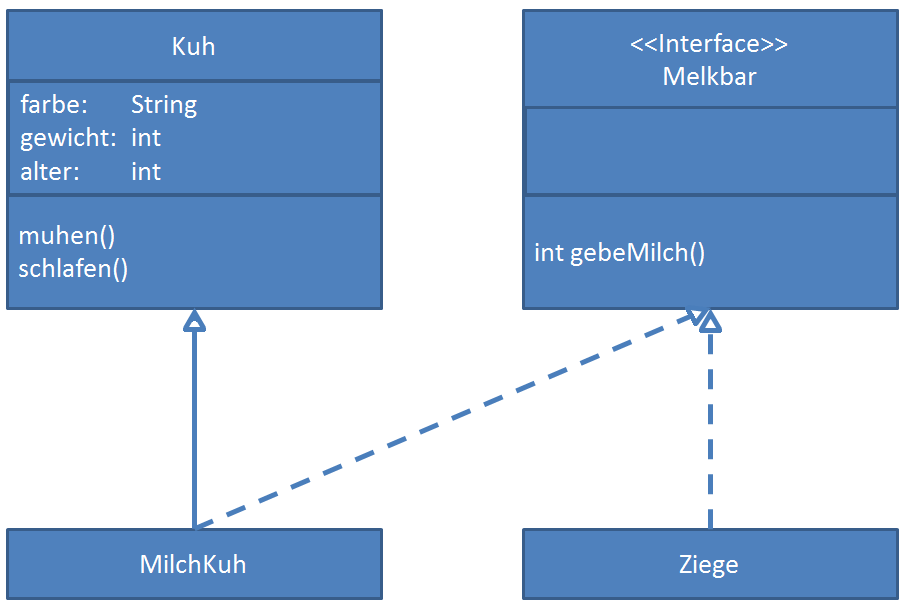
\includegraphics[width=0.8\textwidth,
			keepaspectratio=true]{bilder/milchkuh.png}
		\end{center}
\end{frame}

\begin{frame}[fragile]
	\frametitle{Interfaces in Aktion}
	\begin{columns}
	\begin{column}{0.5\textwidth}
		  Ziegen und K\"uhe k\"onnen jetzt
		  gemeinsam als melkbare Objekte behandelt
		  werden
	\end{column}
	\begin{column}{0.5\textwidth}
		\begin{lstlisting}
			Melkbar[] zuMelken = new Melkbar[2];
			int gesamtMilch = 0;
			
			MilchKuh frida = new MilchKuh();
			Ziege susi = new Ziege();
			
			zuMelken[0] = frida;
			zuMelken[1] = susi;
			
			for(int i = 0; i < zuMelken.length; i++){
				gesamtMilch += zuMelken[i].gebeMilch();
			}
		\end{lstlisting}
	\end{column}
	\end{columns}
\end{frame}

\begin{frame}
	\frametitle{Zeit f\"ur eine \"Ubung}
	\center
	
\includegraphics[width=0.8\textwidth,
	keepaspectratio=true]{bilder/uebung.png}
\end{frame}